\documentclass{article}
\usepackage{graphicx}
\usepackage[margin=1.5cm]{geometry}
\usepackage{amsmath}

\begin{document}

\title{Thursday Reading Assessment: Unit 5, Field Induction and Inductance}
\author{Prof. Jordan C. Hanson}

\maketitle

\section{Memory Bank}

\begin{itemize}
\item $\epsilon = -L \frac{\Delta I}{\Delta t}$ ... Faraday's law with induction, $L$.  Think of this as the change in voltage across an inductor.
\item Kirchoff's loop rule: the sum of all changes in voltage around a loop in a circuit must be zero.
\end{itemize}

\section{RL Circuits}

\begin{figure}
\centering
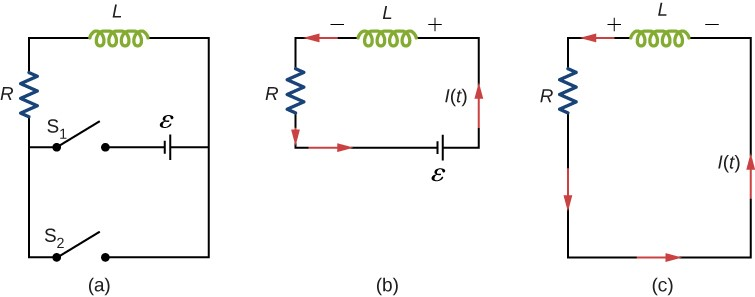
\includegraphics[width=0.5\textwidth]{rl.jpeg}
\caption{\label{fig:rl} A circuit diagram of a DC emf with a resistor, inductor, and two switches.}
\end{figure}

\begin{enumerate}
\item Consider the DC circuit in Fig. \ref{fig:rl}.  There is a battery emf $\epsilon$ connected to a resistor $R$ and and inductor $L$ via switch 1.  Switch 2 simply connects $L$ and $R$.  Suppose we observe the current through the circuit when switch 1 is closed to be
\begin{equation}
i(t) = \frac{\epsilon}{R}\left(1 - \exp(-t/\tau) \right) \label{eq:current}
\end{equation}
(a) In terms of the variables given, what is the current at time $t=0$, when switch 1 is closed? (b) In terms of the variables given, what is the current when $t$ is much larger than $\tau$? (This is like the situation in part (b) of Fig. \ref{eq:current}). \\ \vspace{1cm}
\item After switching out the resistor and inductor independently, we determine that $\tau = L/R$.  (a) What is $\tau$ when $R = 1$ k$\Omega$, and $L = 0.2$ Henries?  (The units should be seconds).  (b) What will the time constant $\tau$ be if we double $R$ and quadruple $L$? \\ \vspace{1cm}
\item Now we return to experimenting, to find out what happens when switch 2 is closed and switch 1 is opened. We do this after switch 1 has been closed for a long time, so that initially, $i \approx \epsilon/R$. The equation is observed to be
\begin{equation}
i(t) = \frac{\epsilon}{R}\exp(-t/\tau)
\end{equation}
What time passes before the current is reduced to half of its original value?
\end{enumerate}
\end{document}
